% **************************************************************************************************
% ** SPSC Report and Thesis Template
% **************************************************************************************************
%
% ***** Authors *****
% Daniel Arnitz, Paul Meissner, Stefan Petrik, Dietmar Malli, Johanna Rock
% Signal Processing and Speech Communication Laboratory (SPSC)
% Graz University of Technology (TU Graz), Austria
%
% ***** Changelog *****
% 0.1   2010-01-25   extracted from report template by Daniel Arnitz (not ready yet)
% 0.2   2010-02-08   added thesis titlepage and modified layout (not ready yet)
% 0.3   2010-02-18   added TUG logo and statutory declaration
% 0.4   2010-02-18   moved the information fields below % **************************************************************************************************
% ** SPSC Report and Thesis Template
% **************************************************************************************************
%
% ***** Authors *****
% Daniel Arnitz, Paul Meissner, Stefan Petrik, Dietmar Malli
% Signal Processing and Speech Communication Laboratory (SPSC)
% Graz University of Technology (TU Graz), Austria
%
% ***** Changelog *****
% 0.1   2010-05-30   some option updates for scrreprt (newer versions)
% 0.2   2010-06-05   split in packages for thesis and report; removed old scrreprt options,
%                    set header to two lines plus adapted geometry
% 0.3   2010-09-13   cite, fixltx2e, [latin1]{inputenc} only for DE, fixed scrreprt options,
%                    paralist, calc, setspace, wrapfig
% 0.4   2011-01-18   scrartcl->scrbook, \Twosided now {true,false}, T1 fontenc for de (hyphenation)
% 0.5   2011-03-31   removed flafter (for top placement)
% 0.6   2011-04-29   added option noadjust to cite (do not set space before \cite automatically)
%                    hmarginratio=3:2 (before: 2:1), voffset=2mm (3mm), added quotchap
% 0.7   2011-12-17   varioref now also works for german text (bug reported by Angelika Kern)
% 0.8   2012-07-27   added option to control paper size (via \PaperSize)
% 0.9   2017-10-31   Removed doubled/copied code which does the same
%                    Added usage of imakeindex with index style file supplied in this template
%                    and removed warning from main.tex
%                    Added enabling of KOMA-Script draft mode if desired by user
%                    fontenc should be loaded before inputenc, because it generates a list parsed by
%                    inputenc [1].
%                    Only load utf8 characters which also can be displayed. (inputenc utf8 instead
%                    of utf8x [2])
%                    Removed cite
%                    Moved hyperref into my package list.. Should always be nearly the last
%                    package called/imported to avoid problems.
%                    Moved documentclass into separate file to have global packages list.
% 1.0   2018-05-01   Added parameter for framed links in hyperref.
%                    
%                    
%
% ***** Todo *****
%
%
% ***** Knowledge sources *****
% [1]https://tex.stackexchange.com/questions/97252/in-which-order-should-i-load-inputenc-and-fontenc
% [2]https://tex.stackexchange.com/questions/13067/utf8x-vs-utf8-inputenc
% **************************************************************************************************

% master
\usepackage{fixltx2e}% LaTeX 2e bugfixes
\usepackage{ifthen}% for optional parts
\ifthenelse{\equal{\PaperSize}{a4paper}}{
\usepackage[paper=\PaperSize,twoside=\Twosided,%
textheight=246mm,%
textwidth=160mm,%
heightrounded=true,% round textheight to multiple of lines (avoids overfull vboxes)
ignoreall=true,% do not include header, footer, and margins in calculations
marginparsep=5pt,% marginpar only used for signs (centered), thus only small sep. needed
marginparwidth=10mm,% prevent margin notes to be out of page
hmarginratio=2:1,% set margin ration (inner:outer for twoside) - (2:3 is default)
]{geometry}}{}%
\ifthenelse{\equal{\PaperSize}{letterpaper}}{
\usepackage[paper=\PaperSize,twoside=\Twosided,%
textheight=9in,%
textwidth=6.5in,%
heightrounded=true,% round textheight to multiple of lines (avoids overfull vboxes)
ignoreheadfoot=false,% do not include header and footer in calculations
marginparsep=5pt,% marginpar only used for signs (centered), thus only small sep. needed
marginparwidth=10mm,% prevent margin notes to be out of page
hmarginratio=3:2,% set margin ration (inner:outer for twoside) - (2:3 is default)
]{geometry}}{}%
\ifthenelse{\equal{\DocumentLanguage}{en}}{\usepackage[T1]{fontenc}\usepackage[utf8]{inputenc}\usepackage[USenglish]{babel}}{}%
\ifthenelse{\equal{\DocumentLanguage}{de}}{\usepackage[T1]{fontenc}\usepackage[utf8]{inputenc}\usepackage[ngerman]{babel}}{}%
\usepackage[%
headtopline,plainheadtopline,% activate all lines (header and footer)
headsepline,plainheadsepline,%
footsepline,plainfootsepline,%
footbotline,plainfootbotline,%
automark% auto update \..mark
]{scrlayer-scrpage}% (KOMA)
\usepackage{imakeidx}
\usepackage[]{caption}% customize captions
%\usepackage{subcaption}
\usepackage{multicol}% multi-column layout
\usepackage{setspace}% (properly) set linespreads
\usepackage[stable,bottom,hang,splitrule,multiple]{footmisc}% customize footnotes

% text
\ifthenelse{\equal{\DocumentLanguage}{en}}{\usepackage{varioref}}{}% improved references
\ifthenelse{\equal{\DocumentLanguage}{de}}{\usepackage[german]{varioref}}{}% improved references
\usepackage{xcolor}% e.g., for color boxes
\usepackage{rotating}% to rotate objects
\usepackage{gensymb}% symbols (perthousand, Celsius, ...)
\usepackage[right]{eurosym}% euro symbol on the right side (51 EUR)
\usepackage[normalem]{ulem}% cross-out, strike-out, underlines (normalem: keep \emph italic)
%\usepackage[safe]{textcomp}% loading in safe mode to avoid problems (see LaTeX companion)
%\usepackage[geometry,misc]{ifsym}% technical symbols
\usepackage{remreset}%\@removefromreset commands (e.g., for continuous footnote numbering)
\usepackage{paralist}% extended list environments
% \usepackage[Sonny]{fncychap}
\usepackage[avantgarde]{quotchap}

% math
\usepackage{amsmath,amssymb,amstext,bm}% math packages
\usepackage{mathcomp}% symbols (perthousand, ...) in math mode


% graphics
\usepackage{graphicx}% use simple graphics
\usepackage{subfigure}% subfigures (a),(b),(c)... within figures
% \usepackage{flafter}% place floats always after reference
\usepackage{placeins}% preventing floats from crossing a barrier
\usepackage{float}% to place floats !HERE!
\usepackage{psfrag}% replace text in eps figures
\usepackage{wrapfig}% inline graphics
\usepackage[export]{adjustbox}


% tables
\usepackage{hhline}% hline doesn't work with colored columns, so using hhline
\usepackage{longtable}% for tables longer than one page
\usepackage{dcolumn}% for number alignment in tables
\usepackage{colortbl}% color in tables


% listings
%\usepackage{alltt}% verbatim environment with commands available
\usepackage{listings}% program code listings


% other
\usepackage{layout}% graphical page layout (spacings)
\usepackage{xspace}% add space after macros if not followed by punctuation character
\usepackage{calc}% online calculations
\makeindex[options=-s ./base/index.sty]% used for index creation

%%%%%%%%%%%%%%%%%%%%%%%%%%%%%%%%%%%
% additions by Dietmar Malli 2017 %
%%%%%%%%%%%%%%%%%%%%%%%%%%%%%%%%%%%
\usepackage{scrhack}              %Fix for: Koma Warning: \float@addtolists detected!
\usepackage{lmodern}              %use modern font
\usepackage{tabularx}             %Special table environment (Table over whole \textwidth)
\usepackage{rotating}             %landscape (also landscape tables combined with tabularx)
\usepackage[hyphens]{url}         %\url command
\usepackage{mdwlist}              %list extensions
\ifthenelse{\equal{\DocumentLanguage}{de}}
{
  \usepackage[german]{fancyref}   %Bessere Querverweise
  \usepackage[locale=DE,          %Zahlen und SI Einheiten
  binary-units=true]{siunitx}     %Zahlen und SI Einheiten => Binary units aktivieren...
  \usepackage[autostyle=true,     %Anführungszeichen und Übersetzung der Literaturverweise
  german=quotes]{csquotes}        %Anführungszeichen und Übersetzung der Literaturverweise
}
{
  \usepackage[english]{fancyref}  %Bessere Querverweise
  \usepackage[locale=USA,         %Zahlen und SI Einheiten
  binary-units=true]{siunitx}     %Zahlen und SI Einheiten => Binary units aktivieren...
  \usepackage[autostyle=true]     %Anführungszeichen und Übersetzung der Literaturverweise
  {csquotes}
}
\sisetup{detect-weight=true, detect-family=true} %format like surrounding environment
%extending fancyref for listings in both languages:
\newcommand*{\fancyreflstlabelprefix}{lst}
\fancyrefaddcaptions{english}{%
  \providecommand*{\freflstname}{listing}%
  \providecommand*{\Freflstname}{Listing}%
}
\fancyrefaddcaptions{german}{%
  \providecommand*{\freflstname}{Listing}%
  \providecommand*{\Freflstname}{Listing}%
}
\frefformat{plain}{\fancyreflstlabelprefix}{\freflstname\fancyrefdefaultspacing#1}
\Frefformat{plain}{\fancyreflstlabelprefix}{\Freflstname\fancyrefdefaultspacing#1}
\frefformat{vario}{\fancyreflstlabelprefix}{%
  \freflstname\fancyrefdefaultspacing#1#3%
}
\Frefformat{vario}{\fancyreflstlabelprefix}{%
  \Freflstname\fancyrefdefaultspacing#1#3%
}

\sisetup{separate-uncertainty}    %enable uncertainity for siunitx
\sisetup{multi-part-units=single} %uncertainity formatting (single, brackets, repeat)
\DeclareSIUnit\permille{\text{\textperthousand}} %add \permille to siunitx
\usepackage{xfrac}                %Schönere brüche für SI Einheiten
\sisetup{per-mode=fraction,       %Bruchstriche bei SI Einheiten aktivieren
fraction-function=\sfrac}         %xfrac als Bruchstrichfunktion verwenden
\usepackage[scaled=0.78]{inconsolata}%Schreibmaschinenschrift für Quellcode

\usepackage[backend=biber,        %Literaturverweiserweiterung Backend auswählen
bibencoding=utf8,                 %.bib-File ist utf8-codiert...
maxbibnames=99,                   %Immer alle Authoren in der Bibliographie darstellen...
style=ieee
]{biblatex}
%\bibliography{bib/bibliography.bib}  %veraltet --> use \addbibresource instead
\addbibresource{bib/bibliography.bib}

\ifthenelse{\equal{\FramedLinks}{true}}
{
  \usepackage[%
  breaklinks=true,% allow line break in links
  colorlinks=false,% if false: framed link
  linkcolor=black,anchorcolor=black,citecolor=black,filecolor=black,%
  menucolor=black,urlcolor=black,bookmarksnumbered=true]{hyperref}% hyperlinks for references
}
{
  \usepackage[%
  breaklinks=true,% allow line break in links
  colorlinks=true,% if false: framed link
  linkcolor=black,anchorcolor=black,citecolor=black,filecolor=black,%
  menucolor=black,urlcolor=black,bookmarksnumbered=true]{hyperref}% hyperlinks for references
}

\setcounter{biburlnumpenalty}{100}%Urls in Bibliographie Zeilenbrechbar machen
\setcounter{biburlucpenalty}{100} %Urls in Bibliographie Zeilenbrechbar machen
\setcounter{biburllcpenalty}{100} %Urls in Bibliographie Zeilenbrechbar machen

\usepackage[acronym,nomain]{glossaries}%Abkürzungsverzeichnis ohne Glossar
\makeglossaries                   %Paket verwenden

%\newacronym{label}{Abkürz.}{Langvers.}
%\newacronym[shortplural=Abk.(Plural),longplural=Langvers.(Plural)]{label}{Abk.}{Langvers.}
%TODO: capitalize or all lower case?
\newacronym{mir}{MIR}{music information retrieval}
\newacronym{ml}{ML}{machine learning}
\newacronym{mfcc}{MFCC}{mel-frequency cepstral coefficients}
\newacronym{ir}{IR}{instrument recognition}
\newacronym{dnn}{DNN}{deep neural network}
\newacronym{cnn}{CNN}{convolutional neural network}
\newacronym{gpu}{GPU}{graphics processing unit}
\newacronym{cv}{CV}{computer vision}
\newacronym{relu}{ReLU}{rectified linear unit}
\newacronym{stft}{STFT}{short-time fourier transform}
\newacronym{dft}{DFT}{discrete fourier transform}
\newacronym{dct}{DCT}{discrete cosine transform}
\newacronym{roc}{ROC}{receiver operating characteristic}
\newacronym{pr}{PR}{precision-recall}
\newacronym{rocauc}{ROC-AUC}{area under the receiver operating characteristic curve}
\newacronym{prauc}{PR-AUC}{area under the precision-recall curve}
\newacronym{rms}{RMS}{root mean square}
\newacronym{lkfs}{LKFS}{loudness, k-weighted, relative to full scale}
\newacronym{lufs}{LUFS}{loudness units relative to full scale}
\newacronym{zcr}{ZCR}{zero-crossing rate}
\newacronym{mse}{MSE}{mean squared error}
\newacronym{rmse}{RMSE}{root mean squared error}
\newacronym{mae}{MAE}{mean absolute error}                  %Acronyme laden

\ifthenelse{\equal{\DocumentLanguage}{de}}
{
  \deftranslation[to=ngerman]       %Dem Paket babel den deutschen Abkürzungsverzeichnis-Kapitelnamen
  {Acronyms}{Abkürzungsverzeichnis} %beibringen
}{}

% misc
\usepackage{datetime}
\newdateformat{monthyeardate}{%
	\monthname[\THEMONTH], \THEYEAR}
 (encoding...)
% 0.5   2010-03-02   added \ShortTitle to fix problems with long thesis titles
%                    added \ThesisType (makes the template suitable for MSc, BSc, PhD, ... Thesis)
% 0.6   2010-06-05   added pagestyle and pagenumbering after frontmatter, packages has now type
% 0.7   2010-09      \Advisors -> \Assessors, inserted frontmatter for thesis
% 0.8   2010-11      added examples
% 0.9   2011-04      \Twosided now {true,false}, scrbook for thesis (\front-, \main-, \backmatter)
%                    added \SpecialNote for titlepage (funding, etc.), added type "homework"
% 0.10  2011-10-18   fixed two typos in \bibliographystyle{} (bug reported by Michael Tauch)
% 0.11  2011-11-09   fixed/modified preamble (bug reported by Michael Tauch)
% 0.12  2012-07-20   added ./base/opt_macros to deal with optional macros
% 0.13  2012-07-27   added \PaperSize
% 0.14  2017-11-03   Fixed thispagestyle issue
%                    Implemented automatic setting of correct page number after switching from
%                    roman numbering back to normal numbering
%                    Implemented \DraftText hack
%                    Moved makeindex from external programm to newer stuff (package...)
%                    Made confidential dependent from \DraftText
%                    Made OptDraftMode and DisplayContentBoxes dependet from \DraftText
%                    Included some syntax formatting definitions
%                    Fixed wrong usage of scrbook class and \emptydoublepage mess... One should
%                    NOT need to adjust/tweak the layout by hand. That's what latex is for...
%                    Replaced bibtex with more modern biblatex (utf8 support in bibliography...)
%                    Added \printbibliography, \listoffigures, \listoftables and 
%                    \printglossary[type=\acronymtype]
%                    Renewed and extended Introduction/Usage
% 0.15  2018-03-20   Homework and report now compileable again. Fixed a missing if.
% 0.16	2018-08-08	 fixed/modified title according to official TUG template
% 0.17	2018-08-09	 updated placeholder commands for new title page
%
% ***** Todo *****
%
% **************************************************************************************************
% basic setup
\newcommand{\DocumentType}{thesis} % "thesis" / "report" / "homework"
\newcommand{\DocumentLanguage}{en} % "en" / "de"
\newcommand{\PaperSize}{a4paper} % "a4paper" / "letterpaper"
\newcommand{\Twosided}{true} % "true" / "false" (=Duplex...)
\newcommand{\FramedLinks}{false} %"true" / "false"

% **************************************************************************************************
% template setup -- do not change these unless you know what you are doing!
% **************************************************************************************************
% ** SPSC Report and Thesis Template
% **************************************************************************************************
%
% ***** Authors *****
% Daniel Arnitz, Paul Meissner, Stefan Petrik, Dietmar Malli
% Signal Processing and Speech Communication Laboratory (SPSC)
% Graz University of Technology (TU Graz), Austria
%
% ***** Changelog *****
% 0.1   2017-10-31   Copied from packages_thesis.tex rev 0.8
%                    Used \openright and removed senseless usages of \emptydoublepage
%
% ***** Todo *****
%
%
% **************************************************************************************************

\documentclass[%
a4paper,           % ATTENTION: geometry package in packages.tex
twoside=\Twosided, % ATTENTION: geometry package in packages.tex
openright,% begin chapters with new right page (openright) or don't care (openany)
11pt,%
fleqn,% equations not centered, but on the left side
captions=tablesignature,% captions below tables
numbers=noenddot,% do not generate point at the end of section numbers (e.g. 1.4.5 instead of 1.4.5.)
headlines=2,% we need two lines in header plus some additional space
final,%
]{scrbook}% (KOMA)

% **************************************************************************************************
% ** SPSC Report and Thesis Template
% **************************************************************************************************
%
% ***** Authors *****
% Daniel Arnitz, Paul Meissner, Stefan Petrik, Dietmar Malli
% Signal Processing and Speech Communication Laboratory (SPSC)
% Graz University of Technology (TU Graz), Austria
%
% ***** Changelog *****
% 0.1   2010-05-30   some option updates for scrreprt (newer versions)
% 0.2   2010-06-05   split in packages for thesis and report; removed old scrreprt options,
%                    set header to two lines plus adapted geometry
% 0.3   2010-09-13   cite, fixltx2e, [latin1]{inputenc} only for DE, fixed scrreprt options,
%                    paralist, calc, setspace, wrapfig
% 0.4   2011-01-18   scrartcl->scrbook, \Twosided now {true,false}, T1 fontenc for de (hyphenation)
% 0.5   2011-03-31   removed flafter (for top placement)
% 0.6   2011-04-29   added option noadjust to cite (do not set space before \cite automatically)
%                    hmarginratio=3:2 (before: 2:1), voffset=2mm (3mm), added quotchap
% 0.7   2011-12-17   varioref now also works for german text (bug reported by Angelika Kern)
% 0.8   2012-07-27   added option to control paper size (via \PaperSize)
% 0.9   2017-10-31   Removed doubled/copied code which does the same
%                    Added usage of imakeindex with index style file supplied in this template
%                    and removed warning from main.tex
%                    Added enabling of KOMA-Script draft mode if desired by user
%                    fontenc should be loaded before inputenc, because it generates a list parsed by
%                    inputenc [1].
%                    Only load utf8 characters which also can be displayed. (inputenc utf8 instead
%                    of utf8x [2])
%                    Removed cite
%                    Moved hyperref into my package list.. Should always be nearly the last
%                    package called/imported to avoid problems.
%                    Moved documentclass into separate file to have global packages list.
% 1.0   2018-05-01   Added parameter for framed links in hyperref.
%                    
%                    
%
% ***** Todo *****
%
%
% ***** Knowledge sources *****
% [1]https://tex.stackexchange.com/questions/97252/in-which-order-should-i-load-inputenc-and-fontenc
% [2]https://tex.stackexchange.com/questions/13067/utf8x-vs-utf8-inputenc
% **************************************************************************************************

% master
\usepackage{fixltx2e}% LaTeX 2e bugfixes
\usepackage{ifthen}% for optional parts
\ifthenelse{\equal{\PaperSize}{a4paper}}{
\usepackage[paper=\PaperSize,twoside=\Twosided,%
textheight=246mm,%
textwidth=160mm,%
heightrounded=true,% round textheight to multiple of lines (avoids overfull vboxes)
ignoreall=true,% do not include header, footer, and margins in calculations
marginparsep=5pt,% marginpar only used for signs (centered), thus only small sep. needed
marginparwidth=10mm,% prevent margin notes to be out of page
hmarginratio=2:1,% set margin ration (inner:outer for twoside) - (2:3 is default)
]{geometry}}{}%
\ifthenelse{\equal{\PaperSize}{letterpaper}}{
\usepackage[paper=\PaperSize,twoside=\Twosided,%
textheight=9in,%
textwidth=6.5in,%
heightrounded=true,% round textheight to multiple of lines (avoids overfull vboxes)
ignoreheadfoot=false,% do not include header and footer in calculations
marginparsep=5pt,% marginpar only used for signs (centered), thus only small sep. needed
marginparwidth=10mm,% prevent margin notes to be out of page
hmarginratio=3:2,% set margin ration (inner:outer for twoside) - (2:3 is default)
]{geometry}}{}%
\ifthenelse{\equal{\DocumentLanguage}{en}}{\usepackage[T1]{fontenc}\usepackage[utf8]{inputenc}\usepackage[USenglish]{babel}}{}%
\ifthenelse{\equal{\DocumentLanguage}{de}}{\usepackage[T1]{fontenc}\usepackage[utf8]{inputenc}\usepackage[ngerman]{babel}}{}%
\usepackage[%
headtopline,plainheadtopline,% activate all lines (header and footer)
headsepline,plainheadsepline,%
footsepline,plainfootsepline,%
footbotline,plainfootbotline,%
automark% auto update \..mark
]{scrlayer-scrpage}% (KOMA)
\usepackage{imakeidx}
\usepackage[]{caption}% customize captions
%\usepackage{subcaption}
\usepackage{multicol}% multi-column layout
\usepackage{setspace}% (properly) set linespreads
\usepackage[stable,bottom,hang,splitrule,multiple]{footmisc}% customize footnotes

% text
\ifthenelse{\equal{\DocumentLanguage}{en}}{\usepackage{varioref}}{}% improved references
\ifthenelse{\equal{\DocumentLanguage}{de}}{\usepackage[german]{varioref}}{}% improved references
\usepackage{xcolor}% e.g., for color boxes
\usepackage{rotating}% to rotate objects
\usepackage{gensymb}% symbols (perthousand, Celsius, ...)
\usepackage[right]{eurosym}% euro symbol on the right side (51 EUR)
\usepackage[normalem]{ulem}% cross-out, strike-out, underlines (normalem: keep \emph italic)
%\usepackage[safe]{textcomp}% loading in safe mode to avoid problems (see LaTeX companion)
%\usepackage[geometry,misc]{ifsym}% technical symbols
\usepackage{remreset}%\@removefromreset commands (e.g., for continuous footnote numbering)
\usepackage{paralist}% extended list environments
% \usepackage[Sonny]{fncychap}
\usepackage[avantgarde]{quotchap}

% math
\usepackage{amsmath,amssymb,amstext,bm}% math packages
\usepackage{mathcomp}% symbols (perthousand, ...) in math mode


% graphics
\usepackage{graphicx}% use simple graphics
\usepackage{subfigure}% subfigures (a),(b),(c)... within figures
% \usepackage{flafter}% place floats always after reference
\usepackage{placeins}% preventing floats from crossing a barrier
\usepackage{float}% to place floats !HERE!
\usepackage{psfrag}% replace text in eps figures
\usepackage{wrapfig}% inline graphics
\usepackage[export]{adjustbox}


% tables
\usepackage{hhline}% hline doesn't work with colored columns, so using hhline
\usepackage{longtable}% for tables longer than one page
\usepackage{dcolumn}% for number alignment in tables
\usepackage{colortbl}% color in tables


% listings
%\usepackage{alltt}% verbatim environment with commands available
\usepackage{listings}% program code listings


% other
\usepackage{layout}% graphical page layout (spacings)
\usepackage{xspace}% add space after macros if not followed by punctuation character
\usepackage{calc}% online calculations
\makeindex[options=-s ./base/index.sty]% used for index creation

%%%%%%%%%%%%%%%%%%%%%%%%%%%%%%%%%%%
% additions by Dietmar Malli 2017 %
%%%%%%%%%%%%%%%%%%%%%%%%%%%%%%%%%%%
\usepackage{scrhack}              %Fix for: Koma Warning: \float@addtolists detected!
\usepackage{lmodern}              %use modern font
\usepackage{tabularx}             %Special table environment (Table over whole \textwidth)
\usepackage{rotating}             %landscape (also landscape tables combined with tabularx)
\usepackage[hyphens]{url}         %\url command
\usepackage{mdwlist}              %list extensions
\ifthenelse{\equal{\DocumentLanguage}{de}}
{
  \usepackage[german]{fancyref}   %Bessere Querverweise
  \usepackage[locale=DE,          %Zahlen und SI Einheiten
  binary-units=true]{siunitx}     %Zahlen und SI Einheiten => Binary units aktivieren...
  \usepackage[autostyle=true,     %Anführungszeichen und Übersetzung der Literaturverweise
  german=quotes]{csquotes}        %Anführungszeichen und Übersetzung der Literaturverweise
}
{
  \usepackage[english]{fancyref}  %Bessere Querverweise
  \usepackage[locale=USA,         %Zahlen und SI Einheiten
  binary-units=true]{siunitx}     %Zahlen und SI Einheiten => Binary units aktivieren...
  \usepackage[autostyle=true]     %Anführungszeichen und Übersetzung der Literaturverweise
  {csquotes}
}
\sisetup{detect-weight=true, detect-family=true} %format like surrounding environment
%extending fancyref for listings in both languages:
\newcommand*{\fancyreflstlabelprefix}{lst}
\fancyrefaddcaptions{english}{%
  \providecommand*{\freflstname}{listing}%
  \providecommand*{\Freflstname}{Listing}%
}
\fancyrefaddcaptions{german}{%
  \providecommand*{\freflstname}{Listing}%
  \providecommand*{\Freflstname}{Listing}%
}
\frefformat{plain}{\fancyreflstlabelprefix}{\freflstname\fancyrefdefaultspacing#1}
\Frefformat{plain}{\fancyreflstlabelprefix}{\Freflstname\fancyrefdefaultspacing#1}
\frefformat{vario}{\fancyreflstlabelprefix}{%
  \freflstname\fancyrefdefaultspacing#1#3%
}
\Frefformat{vario}{\fancyreflstlabelprefix}{%
  \Freflstname\fancyrefdefaultspacing#1#3%
}

\sisetup{separate-uncertainty}    %enable uncertainity for siunitx
\sisetup{multi-part-units=single} %uncertainity formatting (single, brackets, repeat)
\DeclareSIUnit\permille{\text{\textperthousand}} %add \permille to siunitx
\usepackage{xfrac}                %Schönere brüche für SI Einheiten
\sisetup{per-mode=fraction,       %Bruchstriche bei SI Einheiten aktivieren
fraction-function=\sfrac}         %xfrac als Bruchstrichfunktion verwenden
\usepackage[scaled=0.78]{inconsolata}%Schreibmaschinenschrift für Quellcode

\usepackage[backend=biber,        %Literaturverweiserweiterung Backend auswählen
bibencoding=utf8,                 %.bib-File ist utf8-codiert...
maxbibnames=99,                   %Immer alle Authoren in der Bibliographie darstellen...
style=ieee
]{biblatex}
%\bibliography{bib/bibliography.bib}  %veraltet --> use \addbibresource instead
\addbibresource{bib/bibliography.bib}

\ifthenelse{\equal{\FramedLinks}{true}}
{
  \usepackage[%
  breaklinks=true,% allow line break in links
  colorlinks=false,% if false: framed link
  linkcolor=black,anchorcolor=black,citecolor=black,filecolor=black,%
  menucolor=black,urlcolor=black,bookmarksnumbered=true]{hyperref}% hyperlinks for references
}
{
  \usepackage[%
  breaklinks=true,% allow line break in links
  colorlinks=true,% if false: framed link
  linkcolor=black,anchorcolor=black,citecolor=black,filecolor=black,%
  menucolor=black,urlcolor=black,bookmarksnumbered=true]{hyperref}% hyperlinks for references
}

\setcounter{biburlnumpenalty}{100}%Urls in Bibliographie Zeilenbrechbar machen
\setcounter{biburlucpenalty}{100} %Urls in Bibliographie Zeilenbrechbar machen
\setcounter{biburllcpenalty}{100} %Urls in Bibliographie Zeilenbrechbar machen

\usepackage[acronym,nomain]{glossaries}%Abkürzungsverzeichnis ohne Glossar
\makeglossaries                   %Paket verwenden

%\newacronym{label}{Abkürz.}{Langvers.}
%\newacronym[shortplural=Abk.(Plural),longplural=Langvers.(Plural)]{label}{Abk.}{Langvers.}
%TODO: capitalize or all lower case?
\newacronym{mir}{MIR}{music information retrieval}
\newacronym{ml}{ML}{machine learning}
\newacronym{mfcc}{MFCC}{mel-frequency cepstral coefficients}
\newacronym{ir}{IR}{instrument recognition}
\newacronym{dnn}{DNN}{deep neural network}
\newacronym{cnn}{CNN}{convolutional neural network}
\newacronym{gpu}{GPU}{graphics processing unit}
\newacronym{cv}{CV}{computer vision}
\newacronym{relu}{ReLU}{rectified linear unit}
\newacronym{stft}{STFT}{short-time fourier transform}
\newacronym{dft}{DFT}{discrete fourier transform}
\newacronym{dct}{DCT}{discrete cosine transform}
\newacronym{roc}{ROC}{receiver operating characteristic}
\newacronym{pr}{PR}{precision-recall}
\newacronym{rocauc}{ROC-AUC}{area under the receiver operating characteristic curve}
\newacronym{prauc}{PR-AUC}{area under the precision-recall curve}
\newacronym{rms}{RMS}{root mean square}
\newacronym{lkfs}{LKFS}{loudness, k-weighted, relative to full scale}
\newacronym{lufs}{LUFS}{loudness units relative to full scale}
\newacronym{zcr}{ZCR}{zero-crossing rate}
\newacronym{mse}{MSE}{mean squared error}
\newacronym{rmse}{RMSE}{root mean squared error}
\newacronym{mae}{MAE}{mean absolute error}                  %Acronyme laden

\ifthenelse{\equal{\DocumentLanguage}{de}}
{
  \deftranslation[to=ngerman]       %Dem Paket babel den deutschen Abkürzungsverzeichnis-Kapitelnamen
  {Acronyms}{Abkürzungsverzeichnis} %beibringen
}{}

% misc
\usepackage{datetime}
\newdateformat{monthyeardate}{%
	\monthname[\THEMONTH], \THEYEAR}

% **************************************************************************************************
% ** SPSC Report and Thesis Template
% **************************************************************************************************
%
% ***** Authors *****
% Daniel Arnitz, Paul Meissner, Stefan Petrik
% Signal Processing and Speech Communication Laboratory (SPSC)
% Graz University of Technology (TU Graz), Austria
%
% ***** Changelog *****
% 0.2   2010-03-02   title in header now \ShortTitle (before: \DocumentTitle)
% 0.3   2010-08      minor modifications to caption setup
% 0.4   2010-09/10   removed changes of \thepart, modified font for \paragraph, minor mod. to captions,
%                    removed \setlength\parindent{0cm}
% 0.5   2011-01      caption: aboveskip=8pt,belowskip=8pt, slight modifications to listings
% 0.6   2011-03-31   modified figure placement ruleset
% 0.7   2011-04-28   added \emptypage, removed \raggedbottom, returned fig. placement to prev. state
% 0.8   2011-08-31   fixed modification of \figurename
% 0.9   2018-08-08   removed top/bottom header/footer lines
%
% ***** Todo *****
%
% **************************************************************************************************



% **************************************************************************************************
% * PAGE
% **************************************************************************************************

% pagestyle
\pagestyle{scrheadings}%
% \setlength\parindent{0cm}% no indentation for first line of new paragraph
% \raggedbottom% do not try to fill pages

% header and footer size
\setheadwidth{text}% set header width to textwidth
\setfootwidth{text}% set footer width to textwidth
\setheadtopline[textwithmarginpar]{0.5pt}% set up separator lines (greater width than text)
\setheadsepline[textwithmarginpar]{0.5pt}
\setfootsepline[textwithmarginpar]{0.5pt}
\setfootbotline[textwithmarginpar]{0.5pt}

% remove top and bottom lines
\setheadtopline{0pt}
\setfootbotline{0pt}

% redefine cleardoublepage...
\makeatletter
\renewcommand{\cleardoublepage}{\clearpage\if@twoside\ifodd\c@page\else\thispagestyle{plain}\hbox{}\newpage\if@twocolumn\hbox{}\newpage\fi\fi\fi}
% ...and define empty double page (e.g., for title sheet)
\newcommand{\emptydoublepage}{\clearpage\if@twoside\ifodd\c@page\else\thispagestyle{empty}\hbox{}\newpage\if@twocolumn\hbox{}\newpage\fi\fi\fi}%
% ...and also an empty single page
\newcommand{\emptypage}{\clearpage\thispagestyle{empty}\hbox{}\newpage\if@twocolumn\hbox{}\newpage\fi}%
\makeatother

% header and footer texts
\clearscrheadfoot % clear everything
\KOMAoptions{headlines=1} % header needs two lines here
% [plain]{actual (scrheadings)}
\ihead[]{}%
\ohead[\ShortTitle]{\footnotesize\headmark}%
\cfoot[\footnotesize\ConfidNote]{\footnotesize\ConfidNote}%
\ofoot[--~~\pagemark~~--]{--~~\pagemark~~--}%



% **************************************************************************************************
% * TEXT
% **************************************************************************************************

% headlines / table-of-contents
% \renewcommand{\thepart}{\Alph{part}}% workaround for table of contents (VIII too long)
\setkomafont{paragraph}{\normalfont\bfseries}

% footnotes
\renewcommand{\footnotemargin}{1.3 em}% footnote marker to body (default 1.8 em)
\renewcommand{\hangfootparindent}{0pt}% no indention for footnotes spanning more than one line

% listof... (listoftables, listoffigures, ...)
% tableof... (tableofcontents, ...)
\makeatletter
%\@dottedtocline{level}{indent}{numwidth}{text}{page}% standard
%\renewcommand\l@part\@dottedtocline{-1}{1.5em}{2.3em}} % ??
% \renewcommand\l@chapter{\@dottedtocline{0}{1.5em}{2.3em}} % ??
% \renewcommand\l@section{\@dottedtocline{1}{1.5em}{3.3em}}% {1}{1.5em}{2.3em}
% \renewcommand\l@subsection{\@dottedtocline{2}{3.8em}{4.2em}}% {2}{3.8em}{3.2em}
% \renewcommand\l@subsubsection{\@dottedtocline{3}{7.0em}{5.1em}}% {3}{7.0em}{4.1em}
% \renewcommand\l@paragraph{\@dottedtocline{4}{10em}{6em}}% {4}{10em}{5em}
% \renewcommand\l@subparagraph{\@dottedtocline{5}{12em}{7em}}% {5}{12em}{6em}
% \renewcommand\l@figure{\@dottedtocline{1}{1.5em}{3.3em}}% {1}{1.5em}{2.3em}
\renewcommand\l@table{\l@figure}%
\renewcommand\l@lstlisting{\l@figure}%
\renewcommand{\@pnumwidth}{1.85em}% page number width (1.55em)
\makeatother%

% continuous footnote numbering
\makeatletter%
\@removefromreset{footnote}{chapter}%
\makeatother%

% label items
\renewcommand{\labelitemi}{\textbullet}%
\renewcommand{\labelitemii}{$\circ$}%
\renewcommand{\labelitemiii}{--}%
\renewcommand{\labelitemiv}{$\mathbf{\cdot}$}%


% **************************************************************************************************
% * FLOATS
% **************************************************************************************************

% placement
%    Warning: setting floatpagefraction too high will lead to pictures and text '
%    moving out of the page when floats HAVE TO be placed (e.g. FloatBarrier)
\renewcommand{\topfraction}{0.9}% allow nearly full float pages for placement t
\renewcommand{\bottomfraction}{0.9}% allow nearly full float pages for placement b
\renewcommand{\floatpagefraction}{0.9}% do not allow half empty float pages for placement p
\renewcommand{\textfraction}{0.1}% allow little text for h, t, and b placement
\setcounter{topnumber}{10}% max. floats with placement t per page
\setcounter{bottomnumber}{10}% max. floats with placement b per page
\setcounter{totalnumber}{20}% max. floats per page
\makeatletter%
\renewcommand{\fps@figure}{hbtp}%
\renewcommand{\fps@table}{hbtp}%
\makeatother%

% tables (generic)
\setlength\minrowclearance{2pt}% for colortbl package

% longtables
\setlongtables% activate long tables
\setlength{\LTleft}{\fill}% center longtables
\setlength{\LTright}{\fill}%
\setlength{\LTpre}{\medskipamount}%
\setlength{\LTpost}{\bigskipamount}%

% captions
\addtokomafont{captionlabel}{\footnotesize\itshape}%
\addtokomafont{caption}{\footnotesize\itshape}%
\ifthenelse{\equal{\DocumentLanguage}{en}}{\renewcaptionname{USenglish}{\figurename}{Figure}}{}%
\ifthenelse{\equal{\DocumentLanguage}{de}}{\renewcaptionname{ngerman}{\figurename}{Abbildung}}{}%
\captionsetup{%
format=hang,% hanging captions
labelformat=simple,% just name and number
labelsep=colon,% colon and space
justification=justified,%
singlelinecheck=true,% center single line captions
font={footnotesize,it},% font style of label and text
margin=0.025\textwidth,% margin left/right of the caption (to textwidth)
indention=0pt,% no further indention (just hanging)
hangindent=0pt,% no further indention (just hanging)}
aboveskip=8pt,% same spacing above and...
belowskip=8pt}% ...below the float (this way tables shouln't be a problem, either)

% code listings
\lstloadlanguages{VHDL,Matlab,[ANSI]C,Java,[LaTeX]TeX}
\lstset{%
%   general
breaklines=true,% automatically break long lines
breakatwhitespace=true,% break only at white spaces
breakindent=1cm,% additional indentation for broken lines
%   positioning
linewidth=\linewidth,% set width of whole thing to \linewidth
xleftmargin=0.1\linewidth,%
%   frame and caption
frame=tlrb,% frame the entire thing
framexleftmargin=1cm,% to include linenumbering into frame
captionpos=b,% caption at bottom
%   format parameters
basicstyle=\ttfamily\tiny,% small true type font
keywordstyle=\color{black},%
identifierstyle=\color{black},%
commentstyle=\color[rgb]{0.45,0.45,0.45},% gray
stringstyle=\color{black},%
showstringspaces=false,%
showtabs=false,%
tabsize=2,%
%   linenumbers
numberstyle=\tiny,%
numbers=left,%
numbersep=3mm,%
firstnumber=1,%
stepnumber=1,% number every line (0: off)
numberblanklines=true%
}

% **************************************************************************************************
% ** SPSC Report and Thesis Template
% **************************************************************************************************
%
% ***** Authors *****
% Daniel Arnitz, Paul Meissner, Stefan Petrik, Dietmar Malli
% Signal Processing and Speech Communication Laboratory (SPSC)
% Graz University of Technology (TU Graz), Austria
%
% ***** Changelog *****
% 0.1   2010-08-09   added \remc and \remq commands, \nxtpar now uses \med- instead of \bigskip
%                    replaced \lastfootnotemark by \oldfootnotemark (generalization),
%                    added \chapternote, set \openingquote to 0.4\textwidth, modified \MAttention,
%                    \xspace for marginpar commands, modified \MDanger and \MQuestion
% 0.2   2010-10-03   added \exp, colors "bk*"
% 0.3   2010-11-16   added \twofigs and \twofigsf
% 0.4   2010-12      added \F (Fourier), \ceil and \floor
% 0.5   2011-01      added chapter/section/figure/table/part reference commands, textrel
% 0.6   2011-03      added \avg, modified bkred, bkgreen, and bkblue colors,
%                    added \medskip to \chapternote, added natural/real/complex/... numbers
%                    added \rapp for references to the appendix
% 0.7   2011-04      removed labels from \new*NoTOC
% 0.8   2012-06      correction of minor typo
% 0.9   2017-11-03   Dropped custom reference commands (replaced with fancyref)
%                    Implemented automatic usage of \emptydoublepage for thesis
%                    Dropped value unit pairs (replaced with siunitx)
%                    Added pwd command to newchapter. Makes no sense to write that by myself...
%                    changed filelisting to using styles instead of predefined language format.
%                    extended filelisting to support other listings environment options
%
% ***** Todo *****
%
% **************************************************************************************************



% **************************************************************************************************
% * SECTIONING AND TEXT
% **************************************************************************************************

% new chapter, section, ... plus a few addons
%   part
\newcommand{\newpart}[2]{\FloatBarrier\cleardoublepage\part{#1}\label{part:#2}}%
%   chapter
\newcommand{\newchapter}[2]{\FloatBarrier\chapter{#1}\label{chp:#2}\renewcommand{\pwd}{#2}}
\newcommand{\newchapterNoTOC}[1]{\FloatBarrier\stepcounter{chapter}\chapter*{#1}}%
%   section
\newcommand{\newsection}[2]{\FloatBarrier\vspace{5mm}\section{#1}\label{sec:#2}}%
\newcommand{\newsectionNoTOC}[1]{\FloatBarrier\vspace{5mm}\stepcounter{section}\section*{#1}}%
%   subsection
\newcommand{\newsubsection}[2]{\FloatBarrier\vspace{3mm}\subsection{#1}\label{sec:#2}}%
\newcommand{\newsubsectionNoTOC}[1]{\FloatBarrier\vspace{3mm}\stepcounter{subsection}\subsection*{#1}}%
%   subsubsection
\newcommand{\newsubsubsection}[2]{\vspace{2mm}\subsubsection{#1}\label{sec:#2}}%
\newcommand{\newsubsubsectionNoTOC}[1]{\vspace{2mm}\stepcounter{subsubsection}\subsubsection*{#1}}%


% next paragraph
\newcommand{\nxtpar}{\par\medskip}

% "stylish" quotes on the right side
\newcommand{\openingquote}[2]{\hfill\parbox[t]{0.4\textwidth}{\itshape\raggedleft{"#1"}\\\footnotesize -- #2}\nxtpar}%

% some information on the right side (sources, ...)
\newcommand{\chapternote}[1]{\vspace*{-\medskipamount}\hfill\parbox[t]{0.8\textwidth}{\itshape\footnotesize\raggedleft#1}\par\medskip}%

% direct quotes
% \newenvironment{directquote}{\nxtpar\hrule}{\hrule}\hfill\litref{#1}{#2}}

% warnings and attention signs in marginpar
\newcommand{\MDanger}{\marginpar{\raisebox{-2mm}{
\includegraphics[height=7mm]{base/MDanger}}}\xspace}%
\newcommand{\MAttention}{\marginpar{\raisebox{-2mm}{
\includegraphics[height=7mm]{base/MAttention}}}\xspace}%
\newcommand{\MHint}{\marginpar{\raisebox{-2.25mm}{
\includegraphics[height=7mm]{base/MHint}}}\xspace}%
\newcommand{\MQuestion}{\marginpar{\raisebox{-2.25mm}{
\includegraphics[height=7mm]{base/MQuestion}}}\xspace}%

% same footnote number as last one
\newcommand{\oldfootnotemark}[1]{\addtocounter{footnote}{-#1}\footnotemark\addtocounter{footnote}{#1-1}}%
%\newcommand{\lastfootnotemark}{\addtocounter{footnote}{-1}\footnotemark}%

% reminders
\newcommand{\reminder}[1]{\colorbox{red}{#1}\xspace}%
\newcommand{\rem}{\reminder{(...)}}% shortcut for the full reminder
\newcommand{\remq}{\reminder{???}}% open question
\newcommand{\remc}{\reminder{[?]}}% open citation
\newcommand{\uc}{\nxtpar\colorbox{yellow}{... under construction ...}\nxtpar}%

% misc
\newcommand{\pwd}{.} % present working directory (can be used to create relativ paths per part, etc.)




% **************************************************************************************************
% * MATH
% **************************************************************************************************

% highlighting
\newcommand{\vm}[1]{\ensuremath{\bm{#1}}}% vector or matrix

% functions
\renewcommand{\exp}[1]{\ensuremath{\text{e}^{#1}}}% exponential
\renewcommand{\ln}[1]{\ensuremath{\text{ln}\!\left(#1\right)}}% natural logarithm
\newcommand{\ld}[1]{\ensuremath{\text{ld}\!\left(#1\right)}}% logarithm base 2
\renewcommand{\log}[1]{\ensuremath{\text{log}\!\left(#1\right)}}% logarithm (base 10)
\newcommand{\logb}[2]{\ensuremath{\text{log}_{#1}\!\left(#2\right)}}% logarithm base ...

% rounding
\newcommand{\round}[1]{\ensuremath{\text{round}\!\left(#1\right)}}% rounding towards next integer
\newcommand{\ceil}[1]{\ensuremath{\left\lceil#1\right\rceil}}% rounding towards infinity
\newcommand{\floor}[1]{\ensuremath{\left\lfloor#1\right\rfloor}}% rounding towards zero

% operators
\newcommand{\E}[1]{\ensuremath{\text{E}\!\left\{#1\right\}}}% expectation operator
\newcommand{\F}[1]{\ensuremath{\mathcal{F}\!\left\{#1\right\}}}% Fourier transform operator
\newcommand{\IF}[1]{\ensuremath{\mathcal{F}^{-1}\!\left\{#1\right\}}}% inverse Fourier transform operator
\newcommand{\var}[1]{\ensuremath{\text{var}\!\left\{#1\right\}}}% variance operator
\newcommand{\cov}[1]{\ensuremath{\text{cov}\!\left\{#1\right\}}}% covariance operator
\newcommand{\corr}[1]{\ensuremath{\text{corr}\!\left\{#1\right\}}}% correlation operator
\newcommand{\avg}[1]{\ensuremath{\text{avg}\!\left\{#1\right\}}}% averaging operator
\newcommand{\avgvar}[1]{\ensuremath{\overline{\text{var}}\!\left\{#1\right\}}}% average variance operator
\renewcommand{\Re}[1]{\ensuremath{\text{Re}\!\left\{#1\right\}}}% real part
\renewcommand{\Im}[1]{\ensuremath{\text{Im}\!\left\{#1\right\}}}% imaginary part

% numbers
\newcommand{\REAL}{\ensuremath{\mathbb{R}}}% real numbers
\newcommand{\NATURAL}{\ensuremath{\mathbb{N}}}% natural numbers
\newcommand{\INTEGER}{\ensuremath{\mathbb{Z}}}% integer numbers (natural numbers plus zero)
\newcommand{\COMPLEX}{\ensuremath{\mathbb{C}}}% complex numbers
\newcommand{\IMAG}{\ensuremath{\mathbb{I}}}% imaginary numbers

% other
\newcommand{\conj}{\ensuremath{^\ast}}% conjugate complex
\newcommand{\transp}{\ensuremath{^\text{T}}}% conjugate (Hermitian) transpose
\newcommand{\mtx}[2]{\left[\ensuremath{\begin{array}{#1}#2\end{array}\right]}}%vector/matrix
\newcommand{\isdef}{\ensuremath{\mathrel{:=}}}% definition left->right
\newcommand{\isdefflip}{\ensuremath{\mathrel{=:}}}% definition right->left
\newcommand{\isreq}{\ensuremath{\mathrel{\stackrel{!}{=}}}}% is required
\newcommand{\textrel}[1]{\ensuremath{{\;{#1}\;}}}% relation symbol for in-line equations (fixed spacing)



% **************************************************************************************************
% * FLOATS (FIGURES, TABLES, LISTINGS, ...)
% **************************************************************************************************

% figures without frames
%   standard
\newcommand{\fig}[3]{\begin{figure}\centering\includegraphics[width=\textwidth]{#1}\caption{#2}\label{fig:#3}\end{figure}}%
%   with controllable parameters
\newcommand{\figc}[4]{\begin{figure}\centering\includegraphics[#1]{#2}\caption{#3}\label{fig:#4}\end{figure}}%
%   two subfigures
\newcommand{\twofig}[6]{\begin{figure}\centering%
\subfigure[#2]{\includegraphics[width=0.495\textwidth]{#1}}%
\subfigure[#4]{\includegraphics[width=0.495\textwidth]{#3}}%
\caption{#5}\label{fig:#6}\end{figure}}%
%   two subfigures with labels for each subplot
\newcommand{\twofigs}[8]{\begin{figure}\centering%
\subfigure[#2]{\includegraphics[width=0.495\textwidth]{#1}\label{fig:#8#3}}%
\subfigure[#5]{\includegraphics[width=0.495\textwidth]{#4}\label{fig:#8#6}}%
\caption{#7}\label{fig:#8}\end{figure}}%
%   two subfigures and controllable parameters
\newcommand{\twofigc}[8]{\begin{figure}\centering%
\subfigure[#3]{\includegraphics[#1]{#2}}%
\subfigure[#6]{\includegraphics[#4]{#5}}%
\caption{#7}\label{fig:#8}\end{figure}}%

% framed figures
%   standard
\newcommand{\figf}[3]{\begin{figure}\centering\fbox{\includegraphics[width=\textwidth]{#1}}\caption{#2}\label{fig:#3}\end{figure}}%
%   with controllable parameters
\newcommand{\figcf}[4]{\begin{figure}\centering\fbox{\includegraphics[#1]{#2}}\caption{#3}\label{fig:#4}\end{figure}}%
%   two subfigures
\newcommand{\twofigf}[6]{\begin{figure}\centering%
\fbox{\subfigure[#2]{\includegraphics[width=0.495\textwidth]{#1}}}%
\fbox{\subfigure[#4]{\includegraphics[width=0.495\textwidth]{#3}}}%
\caption{#5}\label{fig:#6}\end{figure}}%
%   two subfigures with labels for each subplot
\newcommand{\twofigsf}[8]{\begin{figure}\centering%
\fbox{\subfigure[#2]{\includegraphics[width=0.495\textwidth]{#1}\label{fig:#8#3}}}%
\fbox{\subfigure[#5]{\includegraphics[width=0.495\textwidth]{#4}\label{fig:#8#6}}}%
\caption{#7}\label{fig:#8}\end{figure}}%
%   two subfigures and controllable parameters
\newcommand{\twofigcf}[8]{\begin{figure}\centering%
\fbox{\subfigure[#3]{\includegraphics[#1]{#2}}}%
\fbox{\subfigure[#6]{\includegraphics[#4]{#5}}}%
\caption{#7}\label{fig:#8}\end{figure}}%

% listings
\newcommand{\filelisting}[5][]{\lstinputlisting[style=#2,caption={#4},label={lst:#5},#1]{#3}}

% preserve backslash for linebreaks in tables (ragged... redefines \\, thus it has to be preserved)
\newcommand{\pbs}[1]{\let\temp=\\#1\let\\=\temp}%


% **************************************************************************************************
% * MISC
% **************************************************************************************************

% slighly darkened colors for text
\definecolor{bkred}{rgb}{0.9,0,0}
\definecolor{bkgreen}{rgb}{0,0.67,0}
\definecolor{bkblue}{rgb}{0,0,0.75}

% **************************************************************************************************

% uncomment to get watermarks:
% \usepackage[first,bottom,light,draft]{draftcopy}
% \draftcopyName{ENTWURF}{160}

% correct bad hyphenation
\hyphenation{}

% switches
\newboolean{OptDraftMode}
\newboolean{DisplayContentBoxes}
% \setboolean{OptDraftMode}{true} % optional draft mode for pixel graphics (speed up generation; add \OptDraft to options)

\ifthenelse{\boolean{OptDraftMode}}
{
	\setboolean{DisplayContentBoxes}{true}
}
{
	\setboolean{DisplayContentBoxes}{false}
}


% **************************************************************************************************
% information fields

% general
\newcommand{\DocumentTitle}{Multi-Instrument Recognition, Mix-Parameter Estimation and Timbre Characterization using Deep Neural Networks}
%\newcommand{\DocumentSubtitle}{Subtitle}
\newcommand{\ShortTitle}{Short Title (Header)} % used in headers (keep short!)
% for thesis: Firstname Surename, current university degree (e.g. BSc)
% for report, homework: Firstname Surename, Mat.Nr.
\newcommand{\DocumentAuthor}{Hannes Bradl}
\newcommand{\DocumentPlace}{Graz}

% FOR THESIS ONLY
% used for the title page and statutory declaration
% one out of: "bachelor's thesis" / "Bachelorarbeit" /
%			  "master's thesis" / "Masterarbeit" /
%			  "diploma thesis" / "Diplomarbeit" /
%			  "doctoral thesis" / "Dissertation"
% ATTENTION: use correct language! Otherwise statutory declaration is faulty.
\newcommand{\ThesisTitle}{master's thesis}
\newcommand{\Institute}{Signal Processing and Speech Communication Laboratory}
\newcommand{\OrganizationsAdditional}{in cooperation with \\[0.2cm] \par sonible GmbH \\ Graz, Austria \\[2.0cm] \par} 
\newcommand{\Supervisors}{Univ.-Prof. Dipl.-Ing. Dr.mont Franz Pernkopf} % Supervisor 1 \\ Supervisor 2 ...
\newcommand{\SpecialNote}{This work was funded by the Austrian Research Promotion Agency (FFG) under grant 123456 (TODO: find out the grant number).}

% FOR REPORT ONLY
%revision numbers
\newcommand{\RevPrefix}{alpha~}
\newcommand{\RevLarge}{1}
\newcommand{\RevSmall}{0}

% confidential? (can of course also be used for other messages/notes)
\newcommand{\ConfidNote}{\ifthenelse{\boolean{OptDraftMode}}{
		\textbf{DRAFT}, \today,
]}{
		%\textbf{CONFIDENTIAL}
}}


% **************************************************************************************************
% ** SPSC Report and Thesis Template
% **************************************************************************************************
%
% ***** Authors *****
% Daniel Arnitz, Paul Meissner, Stefan Petrik
% Signal Processing and Speech Communication Laboratory (SPSC)
% Graz University of Technology (TU Graz), Austria
%
% ***** Changelog *****
% 0.1   2012-07-20   \OptDraft and \ContentBox
%
% ***** Todo *****
%
% **************************************************************************************************


% optional boxes with intended contents or other comments (can be switched on/off)
\newcommand{\ContentBox}[2]{\ifthenelse{\boolean{DisplayContentBoxes}}{\FloatBarrier\nxtpar\colorbox{yellow}{\parbox{\textwidth}{\footnotesize#1\par\hrulefill\par Number of pages: #2}}\nxtpar}{}}

% optional draft mode for large graphics (add \OptDraft to parameters for \includegraphics)
\ifthenelse{\boolean{OptDraftMode}}{\newcommand{\OptDraft}{draft}}{\newcommand{\OptDraft}{keepaspectratio}}

% variable for page numbering
\newcounter{mypageno}
% **************************************************************************************************
\begin{document}
% **************************************************************************************************
% ====================================================================
%    The author of this file licenses it to you under the Apache
%    License, Version 2.0. You may obtain a copy of the License at
%
%      http://www.apache.org/licenses/LICENSE-2.0
%
%    Unless required by applicable law or agreed to in writing,
%    software distributed under the License is distributed on an
%    "AS IS" BASIS, WITHOUT WARRANTIES OR CONDITIONS OF ANY
%    KIND, either express or implied.  See the License for the
%    specific language governing permissions and limitations
%    under the License.
% ====================================================================
%%%%%%%%%%%%%%%%%%%%%%%%%%%%%%%%%%%%%%%%%%%%%%%%%%%%%%%%%%%%%
% lstlisting syntax formatting (Dietmar Malli (2017-10-31)) %
%%%%%%%%%%%%%%%%%%%%%%%%%%%%%%%%%%%%%%%%%%%%%%%%%%%%%%%%%%%%%
%Farbdefinitionen
\definecolor{light-gray}{gray}{0.45}

%Umlaute im source:
\lstset{literate=%
    {Ö}{{\"O}}1
    {Ä}{{\"A}}1
    {Ü}{{\"U}}1
    {ß}{{\ss}}1
    {ü}{{\"u}}1
    {ä}{{\"a}}1
    {ö}{{\"o}}1
    {~}{{\textasciitilde}}1
}

%Aussehen für verschiedene Quellcodelistingsprachen definieren:
\lstdefinestyle{styMatlab}{
  language=Octave,
  columns=flexible,                   %Schreibmaschinenschrift
  basicstyle=\ttfamily,               %Schreibmaschinenschrift
  fontadjust=true,                    %Schreibmaschinenschrift
  showstringspaces=false,             %Leerzeichendarstellung in Strings deaktivieren
  numbers=left,                       %Zeilennummerierung auf der Linken Seite
  numberstyle=\tiny,                  %Kleinere Zeichen für Zeilennummerierung \ttfamily wäre für normale Schreibmasch.
  numbersep=.5em,                     %Abstand der Zahlen vom Source
  breaklines=true,                    %Zeilenumbruch im Code aktivieren
  breakatwhitespace=false,            %Nur bei Leerzeichen Zeilen umbrechen
  frame=single,                       %Umrandung
  basicstyle=\ttfamily,               %Schriftart und Größe für Quellcode
  commentstyle=\color{light-gray},    %Kommentare hellgrau
  keywordstyle=\color{blue},          %Schlüsselwörter blau
  stringstyle=\color{orange},         %Strings Orange
  lineskip={-1.0pt},                  %Zeilenabstand verringern
  %identifierstyle=\color{SkyBlue},   %Identifier hellblau
  %stepnumber=2                       %Nur alle 2 Zeilen Zeilennummerieren...
  %breakautoindent=true               %Automatisches Einrücken nach Zeilenumbruch...
  %backgroundcolor=\color{white}      %Hintergrundfarbe ändern
  %showtabs=true,                     %Würde Tabulatorendarstellung aktivieren
  %showspaces=false,                  %Würde Leerzeichendarstellung aktivieren
  otherkeywords={repmat,mynorm2,mynorm2mm,rows,columns,complex,mod}%Zusätzliche Schlüsselwörter für Syntaxhighlighting angeben
  %Mögliche Parameter für frame:      none|leftline|topline|bottomline|lines|single|shadowbox|L|R
}
\lstdefinestyle{styVerilog}{
  language=Verilog,
  columns=flexible,                   %Schreibmaschinenschrift
  fontadjust=true,                    %Schreibmaschinenschrift
  showstringspaces=false,             %Leerzeichendarstellung in Strings deaktivieren
  numbers=left,                       %Zeilennummerierung auf der Linken Seite
  numberstyle=\tiny,                  %Kleinere Zeichen für Zeilennummerierung \ttfamily wäre für normale Schreibmasch.
  numbersep=.5em,                     %Abstand der Zahlen vom Source
  breaklines=true,                    %Zeilenumbruch im Code aktivieren
  breakatwhitespace=false,            %Nur bei Leerzeichen Zeilen umbrechen
  frame=single,                       %Umrandung
  basicstyle=\ttfamily,               %Schriftart und Größe für Quellcode
  commentstyle=\color{light-gray},    %Kommentare hellgrau
  keywordstyle=\color{blue},          %Schlüsselwörter blau
  stringstyle=\color{orange},         %Strings Orange
  lineskip={-1.0pt}                   %Zeilenabstand verringern
}
\lstdefinestyle{styC}{
  language=C,
  columns=flexible,                   %Schreibmaschinenschrift
  fontadjust=true,                    %Schreibmaschinenschrift
  showstringspaces=false,             %Leerzeichendarstellung in Strings deaktivieren
  numbers=left,                       %Zeilennummerierung auf der Linken Seite
  numberstyle=\tiny,                  %Kleinere Zeichen für Zeilennummerierung \ttfamily wäre für normale Schreibmasch.
  numbersep=.5em,                     %Abstand der Zahlen vom Source
  breaklines=true,                    %Zeilenumbruch im Code aktivieren
  breakatwhitespace=false,            %Nur bei Leerzeichen Zeilen umbrechen
  frame=single,                       %Umrandung
  basicstyle=\ttfamily,               %Schriftart und Größe für Quellcode
  commentstyle=\color{light-gray},    %Kommentare hellgrau
  keywordstyle=\color{blue},          %Schlüsselwörter blau
  stringstyle=\color{orange},         %Strings Orange
  lineskip={-1.0pt}                   %Zeilenabstand verringern
}
\lstdefinestyle{styMakefile}{
  language=make,
  columns=flexible,                   %Schreibmaschinenschrift
  basicstyle=\ttfamily,               %Schreibmaschinenschrift
  fontadjust=true,                    %Schreibmaschinenschrift
  tabsize=4,                          %Tab=4Spaces
  showstringspaces=false,             %Leerzeichendarstellung in Strings deaktivieren
  numbers=left,                       %Zeilennummerierung auf der Linken Seite
  numberstyle=\tiny,                  %Kleinere Zeichen für Zeilennummerierung \ttfamily wäre für normale Schreibmasch.
  numbersep=.5em,                     %Abstand der Zahlen vom Source
  breaklines=true,                    %Zeilenumbruch im Code aktivieren
  breakatwhitespace=false,            %Nur bei Leerzeichen Zeilen umbrechen
  frame=single,                       %Umrandung
  basicstyle=\ttfamily,               %Schriftart und Größe für Quellcode
  keywordstyle=\color{blue},          %Schlüsselwörter blau
  commentstyle=\color{light-gray},    %Kommentare hellgrau
  stringstyle=\color{orange},         %Strings Orange
  lineskip={-1.0pt}                   %Zeilenabstand verringern
}
\lstdefinestyle{styBash}{
  language=bash,
  columns=flexible,                   %Schreibmaschinenschrift
  basicstyle=\ttfamily,               %Schreibmaschinenschrift
  fontadjust=true,                    %Schreibmaschinenschrift
  tabsize=4,                          %Tab=4Spaces
  showstringspaces=false,             %Leerzeichendarstellung in Strings deaktivieren
  numbers=left,                       %Zeilennummerierung auf der Linken Seite
  numberstyle=\tiny,                  %Kleinere Zeichen für Zeilennummerierung \ttfamily wäre für normale Schreibmasch.
  numbersep=.5em,                     %Abstand der Zahlen vom Source
  breaklines=true,                    %Zeilenumbruch im Code aktivieren
  breakatwhitespace=false,            %Nur bei Leerzeichen Zeilen umbrechen
  frame=single,                       %Umrandung
  basicstyle=\ttfamily,               %Schriftart und Größe für Quellcode
  keywordstyle=\color{blue},          %Schlüsselwörter blau
  commentstyle=\color{light-gray},    %Kommentare hellgrau
  stringstyle=\color{orange},         %Strings Orange
  lineskip={-1.0pt}                  %Zeilenabstand verringern
}
\lstdefinestyle{styTOYASM}{
  language=[x86masm]Assembler,
  columns=flexible,                   %Schreibmaschinenschrift
  fontadjust=true,                    %Schreibmaschinenschrift
  showstringspaces=false,             %Leerzeichendarstellung in Strings deaktivieren
  numbers=left,                       %Zeilennummerierung auf der Linken Seite
  numberstyle=\tiny,                  %Kleinere Zeichen für Zeilennummerierung \ttfamily wäre für normale Schreibmasch.
  numbersep=.5em,                     %Abstand der Zahlen vom Source
  breaklines=true,                    %Zeilenumbruch im Code aktivieren
  breakatwhitespace=false,            %Nur bei Leerzeichen Zeilen umbrechen
  frame=single,                       %Umrandung
  basicstyle=\ttfamily,               %Schriftart und Größe für Quellcode
  commentstyle=\color{light-gray},    %Kommentare hellgrau
  keywordstyle=\color{blue},          %Schlüsselwörter blau
  stringstyle=\color{orange},         %Strings Orange
  lineskip={-1.0pt},                  %Zeilenabstand verringern
  morekeywords={LDI, LDA, STI, LD, BZ}%Zusätzliche Schlüsselwörter für Syntaxhighlighting angeben
}
\lstdefinestyle{styJava}{
  language=Java,
  columns=flexible,                   %Schreibmaschinenschrift
  basicstyle=\ttfamily,               %Schreibmaschinenschrift
  fontadjust=true,                    %Schreibmaschinenschrift
  showstringspaces=false,             %Leerzeichendarstellung in Strings deaktivieren
  numbers=left,                       %Zeilennummerierung auf der Linken Seite
  numberstyle=\tiny,                  %Kleinere Zeichen für Zeilennummerierung \ttfamily wäre für normale Schreibmasch.
  numbersep=.5em,                     %Abstand der Zahlen vom Source
  breaklines=true,                    %Zeilenumbruch im Code aktivieren
  breakatwhitespace=false,            %Nur bei Leerzeichen Zeilen umbrechen
  frame=single,                       %Umrandung
  basicstyle=\ttfamily,               %Schriftart und Größe für Quellcode
  keywordstyle=\color{blue},          %Schlüsselwörter blau
  commentstyle=\color{light-gray},    %Kommentare hellgrau
  stringstyle=\color{orange},         %Strings Orange
  lineskip={-1.0pt}                   %Zeilenabstand verringern
}
\lstdefinestyle{styGnuplot}{
  language=Gnuplot,
  columns=flexible,                   %Schreibmaschinenschrift
  basicstyle=\ttfamily,               %Schreibmaschinenschrift
  fontadjust=true,                    %Schreibmaschinenschrift
  showstringspaces=false,             %Leerzeichendarstellung in Strings deaktivieren
  numbers=left,                       %Zeilennummerierung auf der Linken Seite
  numberstyle=\tiny,                  %Kleinere Zeichen für Zeilennummerierung \ttfamily wäre für normale Schreibmasch.
  numbersep=.5em,                     %Abstand der Zahlen vom Source
  breaklines=true,                    %Zeilenumbruch im Code aktivieren
  breakatwhitespace=false,            %Nur bei Leerzeichen Zeilen umbrechen
  frame=single,                       %Umrandung
  basicstyle=\ttfamily,               %Schriftart und Größe für Quellcode
  keywordstyle=\color{blue},          %Schlüsselwörter blau
  commentstyle=\color{light-gray},    %Kommentare hellgrau
  stringstyle=\color{orange},         %Strings Orange
  lineskip={-1.0pt}                   %Zeilenabstand verringern
}
\lstdefinestyle{styPHP}{
  language=PHP,
  columns=flexible,                   %Schreibmaschinenschrift
  basicstyle=\ttfamily,               %Schreibmaschinenschrift
  fontadjust=true,                    %Schreibmaschinenschrift
  showstringspaces=false,             %Leerzeichendarstellung in Strings deaktivieren
  numbers=left,                       %Zeilennummerierung auf der Linken Seite
  numberstyle=\tiny,                  %Kleinere Zeichen für Zeilennummerierung \ttfamily wäre für normale Schreibmasch.
  numbersep=.5em,                     %Abstand der Zahlen vom Source
  breaklines=true,                    %Zeilenumbruch im Code aktivieren
  breakatwhitespace=false,            %Nur bei Leerzeichen Zeilen umbrechen
  frame=single,                       %Umrandung
  basicstyle=\ttfamily,               %Schriftart und Größe für Quellcode
  keywordstyle=\color{blue},          %Schlüsselwörter blau
  commentstyle=\color{light-gray},    %Kommentare hellgrau
  stringstyle=\color{orange},         %Strings Orange
  lineskip={-1.0pt}                   %Zeilenabstand verringern
}

% for thesis: switch to frontmatter (Roman numbering, etc.)
\ifthenelse{\equal{\DocumentType}{thesis}}
{
\frontmatter \pagestyle{plain} \pagenumbering{Roman}
}{}

%title
% **************************************************************************************************
% ** SPSC Report and Thesis Template
% **************************************************************************************************
%
% ***** Authors *****
% Johanna Rock
%
% ***** Changelog *****
% 0.1  2018-08-09   New title page designed after TUGRAZ template for thesis (from https://tu4u.tugraz.at)
%
% ***** Todo *****
%
% **************************************************************************************************

% **************************************************************************************************
\begin{titlepage}
	\begin{center}
		
\includegraphics[width=30mm]{./base/TUGlogo} \\[3.0cm] \par
		
		{\Large\DocumentAuthor} \\[2.0cm] \par
		
		{\scshape\huge\linespread{0.9}\selectfont\DocumentTitle} \\[0.5cm] \par
		{\Large\DocumentSubtitle} \\[2.0cm] \par
		{\scshape\huge\linespread{0.9}\selectfont\ThesisTitle} \\[0.5cm] \par
		
		  \ifthenelse{\equal{\DocumentLanguage}{en}}{
		  	submitted to \\[0.2cm] \par
		  	
		    {\bfseries\large Graz University of Technology} \\[2.0cm] \par
		  	
		    Supervisors \\[0.2cm] \par
		    
		}{}
		\ifthenelse{\equal{\DocumentLanguage}{de}}{
			eingereicht an der \\[0.2cm] \par
		
			{\bfseries\large Technischen Universität Graz} \\[2.0cm] \par
		
			Betreuer \\[0.2cm] \par
		
		}{}
		\Supervisors \\[0.5cm] \par
	
		{\bfseries\large \Institute} \\[2.0cm] \par
	
		\OrganizationsAdditional
		
		\vfill{\flushright \DocumentPlace, \monthyeardate\today}\\
		{\scriptsize\vspace*{3mm}\SpecialNote\vspace*{-8mm}}
		
	\end{center}
\end{titlepage}


% for thesis: abstract, kurzfassung, affidavit and statutory declaration
\ifthenelse{\equal{\DocumentType}{thesis}}
{
  \emptydoublepage
  \addcontentsline{toc}{chapter}{Statutory Declaration}
  % **************************************************************************************************
% ** SPSC Report and Thesis Template
% **************************************************************************************************
%
% ***** Authors *****
% Daniel Arnitz, Paul Meissner, Andreas Laesser, Stefan Petrik
% Signal Processing and Speech Communication Laboratory (SPSC)
% Graz University of Technology (TU Graz), Austria
%
% ***** Changelog *****
% 0.1   2010-02-18   created
% 0.2   2010-03-02   added German declaration
% 0.3   2010-06-05   removed \pagenumbering
% 0.4   2011-04-27   bugfix: \cleardoublepage replaced by \emptydoublepage
% 0.5   2017-10-31   Transformed to utf-8
%                    Removed emptydoublepage => Done in preamble...
%
% ***** Todo *****
% **************************************************************************************************

% English
\ifthenelse{\equal{\DocumentLanguage}{en}}{
\begin{center}\Large\bfseries Statutory Declaration\end{center}\vspace*{1cm}
\noindent I declare that I have authored this thesis independently, that I have not used other than the declared sources$/$resources, and that I have explicitly marked all material which has been quoted either literally or by content from the used sources.
\par\vspace*{4cm}
\centerline{
\begin{tabular}{m{1.5cm}cm{1.5cm}m{3cm}m{1.5cm}cm{1.5cm}}
\cline{1-3} \cline{5-7}
 & date & & & & (signature) &\\
\end{tabular}}
}

% % German
% \ifthenelse{\equal{\DocumentLanguage}{de}}{
% \begin{center}\Large\bfseries Eidesstattliche Erklärung\end{center}\vspace*{1cm}
% Ich erkläre an Eides statt, dass ich die vorliegende Arbeit selbstständig verfasst, andere als die angegebenen Quellen$/$Hilfsmittel nicht benutzt, und die den benutzten Quellen wörtlich und inhaltlich entnommene Stellen als solche kenntlich gemacht habe.
% \par\vspace*{4cm}
% \centerline{
% \begin{tabular}{m{1.5cm}cm{1.5cm}m{3cm}m{1.5cm}cm{1.5cm}}
% \cline{1-3} \cline{5-7}
%  & Graz, am & & & & (Unterschrift) &\\
% \end{tabular}}
% }


  \emptydoublepage
  %\addcontentsline{toc}{chapter}{Acknowledgements}
\begin{center}\Large\bfseries Acknowledgements\end{center}\vspace*{1cm}\noindent
First of all, I would like to thank sonible GmbH for giving me the opportunity to work on this exciting project. I could not have undertaken this journey without you. Although I was totally inexperienced in deep learning, the topic you proposed fascinated me from the beginning. In particular, I'm grateful to Markus Huber for spending many hours with me discussing problems and guiding me through the project.\\

I would like to express my deepest gratitude to Franz Pernkopf for supervising this thesis. His great expertise in machine learning was invaluable whenever I was stuck with a problem.\\

Furthermore, I want to thank my parents for financing my study time and for their support in everything I do. I always took that for granted, but it is not. I'm just starting to realize how much they did for me in the past 30 years.\\

Special thanks should also go to my girlfriend for her patience when I worked long hours, for proof-reading the whole thesis and for everything else she does for me.
  \emptydoublepage
  \addcontentsline{toc}{chapter}{Abstract (English)}
\begin{center}\Large\bfseries Abstract (English)\end{center}\vspace*{1cm}\noindent 
Write some fancy abstract here!
  \emptydoublepage
  %\addcontentsline{toc}{chapter}{Kurzfassung}
\begin{center}\Large\bfseries Kurzfassung
\end{center}\vspace*{1cm}\noindent
Da Musikdatenbanken und private digitale Musiksammlungen in letzter Zeit stark gewachsen sind, wurde die Verwaltung solch großer Datenmengen zu einer anspruchsvollen Aufgabe. Für verschiedene Anwendungen ist es erforderlich, Aufnahmen mit einer bestimmten Instrumentierung abrufen zu können. Darüber hinaus können auch Informationen über die Klangfarbe der einzelnen Instrumente in einem Mix hilfreich sein. Aus diesem Grund wird in dieser Arbeit ein System zur automatischen Identifizierung von Instrumenten in Musikaufnahmen, zur Bestimmung der Lautstärke jedes Instruments und zur Charakterisierung der jeweiligen Klangfarbe vorgeschlagen. Das System besteht aus zwei Hauptbestandteilen -- einem Klassifikator und einer Reihe von Klangfarbenschätzern. Der Klassifikator ist in der Lage 15 Klassen von Instrumenten aus einem Mix zu identifizieren. Anschließend bestimmen die jeweiligen Klangfarbenschätzer eine Reihe von Klangfarbendeskriptoren für jedes in dem Mix vorhandene Instrument. Alle Modelle werden als \glqq Convolutional Neural Networks\grqq{} (CNNs) realisiert, welche Mel-Spektrogramm-Repräsentationen von kurzen Ausschnitten der Musikaufnahmen als Eingangsdaten verwenden. Um auch unterrepräsentierte Klassen zum Trainieren der Modelle nutzen zu können, wurde eine zweistufige hierarchische Taxonomie erstellt, die acht Instrumentenfamilien und sieben zusätzliche spezifische Instrumente umfasst. Das Training aller Modelle wurde in zwei Phasen aufgeteilt: Nach dem Vortraining mit einem Music-Tagging-Datensatz wurden die neuronalen Netze mit drei Multi-Track-Datensätzen neu trainiert. Wir untersuchten verschiedene Transfer-Learning-Methoden und kamen zu dem Schluss, dass die besten Ergebnisse erzielt werden, wenn man eine Feinabstimmung der Convolutional Layers vornimmt. Unsere Trainingsbeispiele wurden \glqq on-the-fly\grqq{} durch das Mischen von Einzelspuren aus den Multi-Track-Daten erzeugt. Zu diesem Zweck wurden zwei verschiedene Mixing-Strategien untersucht. Es stellte sich heraus, dass eine Kombination aus beiden Mixing-Techniken am besten funktioniert. Schließlich wurden der Klassifikator und die Klangfarbenschätzer in separaten Experimenten evaluiert. Für Klassen mit ausreichend Trainingsdaten erzielt der Klassifikator F-Maße, die dem Stand der Technik entsprechen oder diesen übertreffen. Die Klangfarbenschätzer erzielten ebenfalls gute Ergebnisse; die Leistungsfähigkeit dieser Modelle ist jedoch schwer einzuschätzen, da es keine Ground Truth oder andere Arbeiten zu diesem Thema gibt.
  \emptydoublepage
}{}

\tableofcontents

\ifthenelse{\equal{\DocumentType}{thesis}}
{
\emptydoublepage
\setcounter{mypageno}{\value{page}}
\mainmatter \pagestyle{scrheadings} \pagenumbering{arabic}
\setcounter{page}{\value{mypageno}}
}


% **************************************************************************************************
% mainmatter (=content)

\newchapter{Introduction and Usage}{intro}
The SPSC Thesis/Report/Homework Template provides you with several commands that have proven useful in the creation of a thesis. Nonetheless, they are by no means mandatory. You have to decide which methods and commands you find useful and which you don't. Also, if you have a specific command or best-practice approach you found useful: Tell us! If it fits into this template, we will add it. As always: Feedback, bug reports, feature request, \dots, are greatly appreciated! 
% **************************************************************************************************
% **************************************************************************************************
\newsection{Building the template}{intro:building}

To make the build process easier, you can use the provided bash script, i.e. \verb|bash build.sh|. It executes all commands needed for the standard template in the correct order:
\begin{enumerate}
	\item pdflatex
	\item biber
	\item makeglossaries
	\item pdflatex ($2 \times$)
\end{enumerate}

Alternatively you can execute these commands manually or using your favourite tex editor. Note, that you need to rebuild \verb|biber| and \verb|makeglossaries| only after you modified the respective files, otherwise \verb|pdflatex| is sufficient.



% **************************************************************************************************
% **************************************************************************************************
\newsection{Structure of Sections}{intro:sections}

The template provides several pre-defined commands for parts, chapters, sections, subsections, and subsubsections. These commands contain a mandatory argument for the label, and prevent floats (images and tables) to cross part- chapter and section boundaries. \Fref{tab:intro:sections:commands} in \Fref{sec:intro:sections} lists these commands. This is a citation \cite{Mowlaee2016}. LOOL.

\begin{longtable}{l|c|l}
  \textbf{Command} & \textbf{FloatBarrier} & \textbf{Reference As} \\\hline
  \verb|\newpart{Title}{label}| & yes & \verb|\fref{part:label}| \\
  \verb|\newchapter{Title}{label}| & yes & \verb|\fref{chp:label}| \\
  \verb|\newsection{Title}{label}| & yes & \verb|\fref{sec:label}| \\
  \verb|\newsubsection{Title}{label}| & no & \verb|\fref{sec:label}| \\
  \verb|\newsubsubsection{Title}{label}| & no & \verb|\fref{sec:label}| \\
  \caption{Commands to start new parts, chapters, sections, \dots}
  \label{tab:intro:sections:commands}
\end{longtable}






% **************************************************************************************************
% **************************************************************************************************
\newsection{Layout of Files/Directories}{intro:directories}

Bringing order to the chaos of a thesis is always a problem. Especially the file/directory structure can become somewhat huge and make later changes difficult. The command \verb|\pwd| (print working directory) can be used to divide the thesis into smaller parts and make absolute paths (from the main file) unnecessary.

By starting a new chapter with \verb|\newchapter{Introduction}{intro}|, the working directory is set to the subdirectory \verb|intro|. The command \verb|\pwd| can then be used in all file paths (e.g., \verb|\input| or \verb|\includegraphics|) to make sure all files can be loaded without having to define a path. For example, this file is loaded via \verb|\input{\pwd/intro_basics}|.

Consider creating one directory per chapter, and one file per section. This will make it easier to identify the correct file, and also to shift chapters and especially sections. External files (figures, code, \dots) can for example be placed in subdirectories for each chapter.






% **************************************************************************************************
% **************************************************************************************************
\newsection{Floats: Graphics, Tables, and Listings}{intro:floats}



% **************************************************************************************************
\newsubsection{Figures and Tables}{intro:floats:figures}
Even relatively complex figures are easy to create, as you can see from this example. Note that you can refer to \Fref{fig:intro:floats:usage:figure}, but also to the subfigures: \Fref{fig:intro:floats:usage:figure-ex1} and \Fref{fig:intro:floats:usage:figure-ex2}.
\begin{figure}
  \centering
  \subfigure[left side]{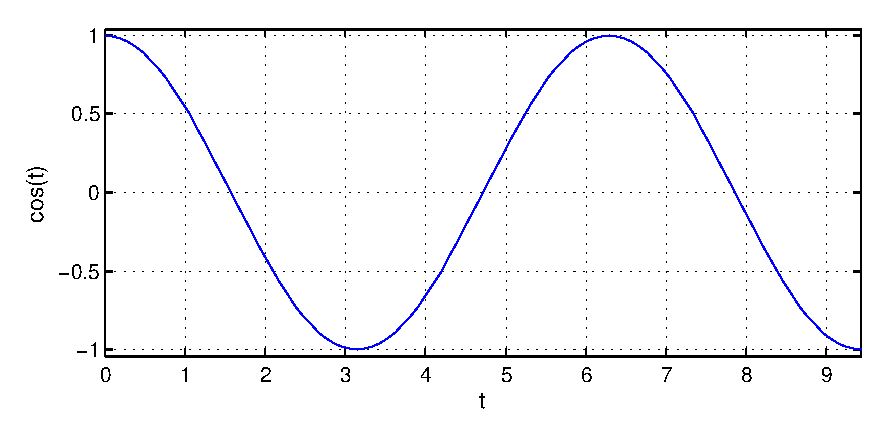
\includegraphics[width=0.495\textwidth]{\pwd/plots/example1}\label{fig:intro:floats:usage:figure-ex1}} \hfill
  \subfigure[right side]{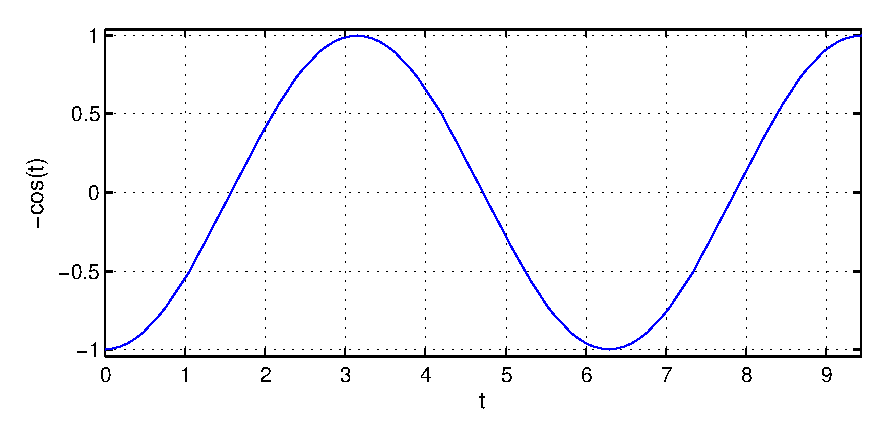
\includegraphics[width=0.495\textwidth]{\pwd/plots/example2}\label{fig:intro:floats:usage:figure-ex2}}
  \caption{Two subplots.}
  \label{fig:intro:floats:usage:figure}
\end{figure}

\noindent To create such two-column figures, the following simplified command can be used:
{
\scriptsize
\begin{verbatim}
  \twofigs{\pwd/plots/example1}{left side}{-ex1}{\pwd/plots/example2}{right side}{-ex2}{Two subplots.}{intro:floats:usage:figure-std}
\end{verbatim}
}
\noindent Reference it using:
\begin{verbatim}
\fref{fig:intro:floats:usage:figure-std}
\end{verbatim}

\noindent See \Fref{tab:intro:floats:figures} for more standardized commands. Captions and labels are mandatory for all these commands.
\begin{longtable}{>{\tiny}l|>{\tiny}p{0.3\textwidth}}
  \normalsize\textbf{Command} & \normalsize\textbf{Description} \\\hline
  \verb|\fig{file}{caption}{label}| & Standard figure, full textwidth. \\\hline
  \verb|\figc{param}{file}{caption}{label}| & Standard figure with controllable parameters for includegraphics. \\\hline
  \verb|\twofig{file_l}{caption_l}{file_r}{caption_r}{caption}{label}| & Two figures, side by side. \\\hline
  \verb|\twofigs{file_l}{caption_l}{add.label_l}{filename_r}{caption_r}{add.label_l}{caption}{label}| & Two figures, side by side, with labels for each subfigure.\\\hline
  \verb|\twofigc{param_l}{file_l}{caption_l}{param_l}{filename_r}{caption_r}{caption}{label}| & Two figures, side by side, with controllable parameters for includegraphics. \\\hline
  \verb|\figf|, \verb|\figcf|, \verb|\twofigf|, \verb|\twofigsf|, \verb|\twofigcf| & Like the above, but with framed figures. \\
  \caption{Standardized commands for figures.}
  \label{tab:intro:floats:figures}
\end{longtable}


% **************************************************************************************************
\newsubsection{Listings}{intro:floats:listings}

A code listing can be included from an external file using:

\begin{verbatim}
\filelisting{styMatlab}{\pwd/plots/matlab.m}{Some matlab code example.}{code-example}
\end{verbatim}

\noindent which looks like this:

\filelisting{styMatlab}{\pwd/plots/matlab.m}{Some matlab code example.}{code-example}

\vspace{5mm}
\noindent To include only certain lines of an external file you can supply option parameters to the listing command like this:

\begin{verbatim}
\filelisting[firstline=3, lastline=6]{styMatlab}{\pwd/plots/matlab.m}{Subset printed.}{param-example}
\end{verbatim}

\vspace{5mm}
\noindent A reference to \Fref{lst:code-example} can be created using

\begin{verbatim}
\Fref{lst:code-example}
\end{verbatim}

\vspace{5mm}
\noindent You can also write code inline using:

\begin{verbatim}
\begin{lstlisting}[style=styMatlab,caption={Some fancy matlab inline code},label={lst:matlabInline}]
clf;
plot(sin(0:1:5));
\end{lstlisting}
\end{verbatim}

% **************************************************************************************************
% **************************************************************************************************
\newsection{Miscellaneous}{intro:misc}

The template also provides several commands that make life easier. The ``reminder'' commands, for example, can be used to \reminder{mark something that should be revised}, but also as a placeholder for leftout parts of a \rem, if there is some open question \remq, or you have to look up some reference \remc. They can easily be found in the source code: Just search for \verb|\rem|. A second group of commands is used to create nice value-unit pairs, such as f=\SI{3}{\kilo\hertz}, \SI{2}{\permille}, or \SI{12.3(4)}{\kilo\gram}.

\vspace{5mm}
Some other examples of SI unit usage:
\begin{itemize}
\item \verb|\SI{1.7e2}{\pico\joule\per\kilo\gram\squared}| will be \SI{1.7e2}{\pico\joule\per\kilo\gram\squared}
\item \verb|\SI{2.8}{\meter\tothe{5}}| to the example: \SI{2.8}{\meter\tothe{5}}
\item \verb|\SI{2 x 3 x 4}{\milli\meter}| volume example: \SI{2 x 3 x 4}{\milli\meter}
\item \verb|\num{12345678}| will be 12 345 678 in german and 12.345.678 in english without changing this source file
\item \verb|\ang{13;14;15}| angle example: \ang{13;14;15}
\item \verb|\SIrange{1}{10}{\m}| Range example: \SIrange{1}{10}{\m}
\end{itemize}

\nxtpar\noindent
Oh, by the way: This section is \uc

\newsection{Citation}{intro:cite}
For citing a new reference, e.g. a book \autocite{Mowlaee2016} or URL \autocite{Example:Url}, you have to add an entry to \verb|./bib/bibliography.bib|.

\newsection{Acronyms}{intro:acn}
Generally, every acronym should be written in full at its first occurence including the short term which is used onwards. To make life easier, you can define acronyms using \verb|\newacronym| in the \verb|acronyms.tex| file and use it with \verb|\gls{label}| (singular) or \verb|\glspl{label}| (plural). So first you define the \gls{pcb} and then only the acronym is used, i.e. \gls{pcb} or \glspl{pcb}.

\newsection{Good to know}{intro:gtk}
\begin{itemize}
\item \verb|There will be~no linebreak between no and be.|
\item \verb|\hspace{10mm} and \vspace{10mm} can be used to create arbitrary amounts of space.|
\item \verb|\hfill will use the rest of the horizontal space in a line.|
\item \verb|- will create a hyphen (Bindestrich)|
\item \verb|-- will create a dash (Gedankenstrich)|
\item \verb|$-$ will create a minus (Mathematisches Minus)|
\item \verb|\url{https://example.org/main.php?param=1&param2=1} (verlinkt)|
\item \verb|\path{C:\Windows\system32\} (verlinkt)|
\end{itemize}

\vspace{5mm}
Syllabification (Silbentrennung):
\begin{itemize}
\item \verb|Syl"-labification would tell Latex another breaking point after the l.| Note that the hyphen will not be printed.
\item \verb|Syl""labification would tell Latex another breaking point after the l.| This time it will be broken without a hyphen. This makes sense for words which already include a hyphen.
\item \verb|\mbox{midnightlunch} forbids latex to break the word completely.|
\end{itemize}

\vspace{5mm}
Enumerations can be done using one of these environments:
\begin{description}
\item[enumerate] using numbers
\item[itemize] using bullets
\item[description] looks like this list
\end{description}

\vspace{5mm}
Referencing prefix list supported by \verb|\fref|:
\begin{description}
\item[chp] chapter
\item[sec] section
\item[fig] figure
\item[tab] table
\item[eq] equation
\item[lst] listing
\item[enum] enumeration
\end{description}

\vspace{5mm}
Enquoting \enquote{stuff} should be done with \verb|\enquote{stuff}|, because it \enquote{translates} the quotes into the style commonly used in the desired language.





\newchapter{Fancy and Advanced}{advanced}
% **************************************************************************************************
% **************************************************************************************************
\newsection{Bringing Style Into Your Thesis}{fancy:style}
\openingquote{They misunderestimated me.}{Guess Who}

The template does not provide too many ``stylish'' commands. One of them created the quote above, the others are intended to mark a part of the text using the margins. You can, for example

\bigskip\bigskip
\dots state that this is dangerous.\MDanger

\bigskip\bigskip
\dots tell the reader to ``better pay attention''.\MAttention

\bigskip\bigskip
\dots mark some central results.\MHint

\bigskip\bigskip
\dots also admit that you're just clueless.\MQuestion








% **************************************************************************************************
% **************************************************************************************************
\newsection{Higher Mathematics}{fancy:math}

Naturally, there are also several commands that should make life easier when dealing with equations. One of the central ideas is to be able to change the general style of something, for example vector/matrix highlighting ($\vm{\phi}$ vs. $\phi$), just by modifying the template command.

\nxtpar\noindent
Here are a few examples. Note that equations (\ref{eq:fancy:math:1}) and (\ref{eq:fancy:math:2}), but also (\ref{eq:fancy:math:3a}) and (\ref{eq:fancy:math:3b}) do not necessarily make sense...
\begin{equation}
  \var{a + b} \isreq \var{a} + \var{b} + 2 \cov{a,b}
  \label{eq:fancy:math:1}
\end{equation}
\begin{equation}\begin{split}
  \vm{H}
  &\isdef \exp{\E{\vm{h}^T \vm{h}}} - \ln{\vm{h}^T \vm{h}} + \log{\vm{h}^T \vm{h}} - \frac{\ld{\vm{h}^T \vm{h}}}{\logb{3}{\vm{h}^T \vm{h}}} \\
  &= \mtx{ccc}{h1 & h2 & \dots \\ 0 & h1 & \dots \\ \vdots & \vdots & \ddots}
  \label{eq:fancy:math:2}
\end{split}\end{equation}
\begin{align}
  \E{ a b\conj c d\conj} &= \E{a b\conj} \cdot \E{c d\conj} + \E{a d\conj} \cdot \E{c b\conj} \label{eq:fancy:math:3a}\\
   \E{a b\conj} \cdot \E{c d\conj} &\neq  \E{a d\conj} \cdot \E{c b\conj} - \E{ a b\conj c d\conj}\label{eq:fancy:math:3b}
\end{align}


% end mainmatter
% **************************************************************************************************

\appendix
\ifthenelse{\equal{\DocumentType}{thesis}}
{
\setcounter{mypageno}{\value{page}}
\frontmatter \pagestyle{plain} \pagenumbering{Roman}
\setcounter{page}{\value{mypageno}}
}{}

\printbibliography[title=References]
\listoffigures
\listoftables
\printglossary[type=\acronymtype]

% \appendix
% \bibliographystyle{./base/IEEEtran}
% \bibliography{_bibliography}


% **************************************************************************************************
% **************************************************************************************************

% place all floats and create label on last page
\FloatBarrier\label{end-of-document}
\end{document}

